\documentclass{classrep}
\usepackage[utf8]{inputenc}
\frenchspacing

\usepackage{graphicx}
\usepackage[usenames,dvipsnames]{color}
\usepackage[hidelinks]{hyperref}
\usepackage{lmodern}
\usepackage{placeins}
\usepackage{url}
\usepackage{amsmath, amssymb, mathtools}
\usepackage{listings}
\usepackage{fancyhdr, lastpage}

\pagestyle{fancyplain}
\fancyhf{}
\renewcommand{\headrulewidth}{0pt}
\cfoot{\thepage\ / \pageref*{LastPage}}
%--------------------------------------------------------------------------------------%
\studycycle{Informatyka, studia dzienne, I st.}
\coursesemester{VI}

\coursename{Komputerowe systemy rozpoznawania}
\courseyear{2019/2020}

\courseteacher{dr hab. inż. Adam Niewiadomski, prof. PŁ}
\coursegroup{poniedziałek, 12:00}

\author{
    \studentinfo{Jan Karwowski}{216793} \and
    \studentinfo{Kamil Kowalewski}{216806}
}

\title{Zadanie 2: Lingwistyczne podsumowania baz danych}

\begin{document}
    \maketitle

    \section{Cel} {
        Celem zadania jest stworzenie aplikacji desktopowej, której główną funkcjonalnością jest lingwistyczna agregacja
        zawartości wybranego zbioru danych. Ma ona za zadanie generować podsumowania lingwistyczne dla wybranych przez
        użytkownika odpowiednio dobranych parametrów tego podsumowania.
    }
%--------------------------------------------------------------------------------------%
    \section{Wprowadzenie} {
        W życiu codziennym ludzie porozumiewają się językiem naturalnym. Język ten, pełen jest
        różnych pojęć nieprecyzyjnych (np. wysoki, biedny, duży), które choć niezwiązane z
        konkretnymi wartościami liczbowymi pozwalają dość skutecznie przenosić informacje. I tak
        kiedy mówi się, że ktoś jest wysoki, to zazwyczaj w danej grupie społecznej ludzie rozumieją
        co autor wypowiedzi ma na myśli i patrząc na tego "wysokiego" sami również klasyfikują go w
        ten sam sposób. Posługiwanie się tym określeniem sprawdza się w praktyce, chociaż nikt
        precyzyjnie nie zdefiniował, kto to jest człowiek wysoki - ile musi mieć wzrostu aby można
        było go takim uznać. Ponadto w rozumieniu "codziennym" ktoś może być wysoki bardziej lub
        mniej (w jakimś stopniu), co również nie zostało nigdzie odgórnie zdefiniowane. Komputery
        natomiast posługują się jedynie określeniami precyzyjnymi, ktoś może być wysoki albo nie,
        wykorzystują logikę klasyczną. Pojawia się więc problem, jak wyrazić pewne informacje, które
        posiada maszyna (w wyniku np. jakichś skomplikowanych obliczeń lub przetwarzania dużych
        zbiorów danych), w języku dobrze zrozumiałym dla człowieka, który na co dzień posługuje się
        określeniami nieprecyzyjnymi.

        Generowanie wyrażeń lingwistycznych przez komputer, w języku quasi-naturalnym, może być
        zreazlizowane za pomocą zbiorów rozmytych. Odpowiednim pojęciom nieprecyzjnym, jak
        wspomniane wcześniej "wysoki", są przyporządkowane zbiory rozmyte, których funkcje
        przynależności zdefiniowane są na podstawie pewnej wiedzy eksperckiej, doświadczenia i
        zdrowego rozsądku. W realizacji tego zadania wyrażenia lingwistyczne są generowane w celu
        stworzenia lingwistycznego podsumowania bazy danych. Na podstawie pewnego zbioru danych
        (obiektów charakteryzowanych przez wartości swoich atrybutów) powstaje zdanie w języku
        quasi-naturalnym, które zawiera informację na temat zawartości tego zbioru. Gdyby zbiór
        zawierał informację na temat parametrów fizycznych grupy ludzi, to takie podsumowanie
        mogłoby brzmieć: "Większość ludzi jest niskich i grubych" i mogło by być bardziej lub mniej
        prawdziwe.

        Generowane będą dwa typy podsumowań - jednopodmiotowe i wielopodmiotowe. Te pierwsze odnoszą
        się do jednego zbioru obiektów a te drugie do wielu (w naszym przypadku dwóch) zbiorów obiektów.
        Podsumowania jednopodmiotowe będą występować w dwóch formach, pierwszej i drugiej:
        \begin{equation}
            Q P \textrm{ are/have } S [T]
        \end{equation}
        \begin{equation}
            Q P \textrm{ being/having } W \textrm{ are/have } S [T]
        \end{equation}
        gdzie $Q$ - kwantyfikator, $P$ - podmiot podsumowania, $W$ - kwalifikator, $S$ - sumaryzator
        (może być złożony), $T$ - wartość pewnej miary lub miar jakości podsumowania. Kwantyfikator
        jest określeniem dotyczącym ilości (np. wiele, mało, ok 1000) i jest definiowany przez
        pewien zbiór rozmyty. Kwalifikator i sumaryzator są określeniami odnoszącymi
        się bezpośrednio do cechy podmiotu (atrybutu) i również są reprezentowane przez zbiory
        rozmyte (np. wysoki, chudy gdyby podmiotem były obiekty typu "człowiek"). Podstawową miarą
        jakości podsumowania jest \emph{degree of truth}, czyli poziom prawdziwości danego
        wyrażenia, obliczany według odpowiedniego wzoru na podstawie zbiorów rozmytych
        reprezentujacych składowe całego wyrażenia oraz na podstawie wartości cech (atrybutów)
        obiektów. Wspomniana miara jest również określana jako T1, istnieją również inne miary (aż
        do T11), które uwzględniają inne właściwości podsumowania. Aby wyrazić ogólną jakość
        podsumowania z uwzględnieniem wszystkich miar jakości (od T1 do T11) można wyliczyć średnią
        ważoną, gdzie suma wszystkich wag musi być równa $1$.
        \begin{equation}
            T = \sum_{i=1}^{11} w_i T_i
        \end{equation}
        gdzie $w_i$ - waga miary jakości $i$, $T_i$ - wartość miary jakości $i$.

        Podsumowanie wielopodmiotowe występuje właściwie w czeterch formach, wykorzystane zostały
        pierwsza, druga i trzecia, których to postacie wyglądają kolejno w następujący sposób:
        \begin{equation}
            Q P_1 \textrm{ compared to } P_2 \textrm{ are/have } S [T]
        \end{equation}
        \begin{equation}
            Q P_1 \textrm{ compared to } P_2 \textrm{ which are/have } W \textrm{ are/have } S [T]
        \end{equation}
        \begin{equation}
            Q P_1 \textrm{ which are/have } W \textrm{ compared to } P_2 \textrm{ are/have } S [T]
        \end{equation}
        gdzie $P_1$ i $P_2$ to kolejno pierwszy i drugi podmiot podsumowania a $W$ to kwalifikator
        odnoszący się w zależności od formy podsumowania do pierwszego lub do drugiego podmiotu.
        Wykorzystaną w tym projekcie miarą jakości podsumowania wielopodmiotowego jest tylko T1,
        której sposób obliczania jest odpowiednio zmodyfikowany. W przypadku, gdy podsumowywany jest
        zbiór danych zawierających tylko jeden typ obiektów, również można tworzyć podsumowania
        wielopodmiotowe.  Wystarczy wyodrębnić rozłączne podzbiory obiektów na podstawie pewnej
        kategorii. Np. w przypadku zbioru obiektów typu człowiek można wyodrębnić dwa podzbiory
        według cechy, którą jest płeć - mężczyźni i kobiety. Powstałe podzbiory mogą być
        wykorzystane do generowania podsumowania wielopodmiotowego, które może wnosić zupełnie nowe
        informacje o zależnościach między kategoriami obiektów, trudne do wykazania z wykorzystaniem
        jedynie podsumowań jednopodmiotowych.
    }
%--------------------------------------------------------------------------------------%
    \section{Opis implementacji} {
        Program został przygotowany w języku Java, w wersji JDK 1.8. Co więcej, technologią
        do obsługi systemu zarządzanie relacyjną bazą danych został wybrany Spring Boot.
        Sam system zarządzania bazą danych był PostgreSQL. Do kontrolowania zależnościami
        projektu został użyty Apache Maven.\\
        W celu zachowania czytelności i możliwości rozbudowy, projekt został podzielony na
        moduły w postaci pakietów: logic, view oraz mode. Ich dokładny opis oraz zawartość
        została przedstawiona poniżej.

        \begin{figure}[!htbp]
            \centering
            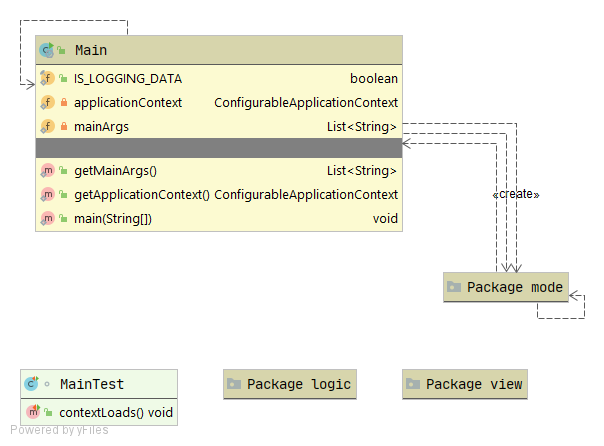
\includegraphics[width=0.6\textwidth]{img/uml/task2.png}
            \caption{Diagram UML}
        \end{figure}
        \FloatBarrier

        \subsection{Pakiet logic} {
            Pakiet zawiera całą logikę aplikacji odpowiadającą za obliczenia rozmyte oraz obsługę bazy danych do
            lokalnego przetwarzania. Najważniejsze dla działania całej aplikacji są podpakiety \emph{fuzzy} oraz
            \emph{model}. Poza tym warte wspomnienia są jeszcze \emph{repository} i \emph{service}, które umożliwiają
            dostęp do analizowanych danych oraz zapis, odczyt i edycję etykiet oraz kwalifikatorów.

            Pakiet \emph{fuzzy} zawiera bibliotekę do obliczeń rozmytych, a diagramy jego klas (podzielonych jeszcze na
            dwa podpakiety - \emph{set} i \emph{linguistic}) zostały przedstawione poniżej. Jak widać pakiet \emph{set}
            zawiera podstawowy model reprezentujący zbiory rozmyte. Klasa FuzzySet jest typem generycznym, może przechowywać
            różne typy obiektów - w przypadku naszej aplikacji będą to oczywiście obiekty klasy Pollution. Klasy pochodne
            FuzzySet reprezentują zbiory z różnymi funkcjami przynależności. Mamy tutaj klasy odpowiadające kolejno
            trójkątnej, trapezoidalnej i gaussowskiej funkcji przynależności, przy czym klasy te wymagają dodatkowego
            parametru pozwalającego mapować obiekty wybranego typu na pewne liczby rzeczywiste (zazwyczaj wartość wybranego
            atrybutu). Istnieje również klasa IntersectionFuzzySet, której instancje reprezentują wyniki iloczynu zbiorów
            rozmytych. Aby wykonać taką operację trzeba po prostu stworzyć obiekt właśnie tej klasy. Ten charakterystyczny
            sposób implementacji operacji na zbiorach rozmytych wynika z faktu, że chcemy uczynić wszystkie klasy z tego
            pakietu serializowalne a różnią się one implementacją funkcji przynależności, nie zaś wartościami pól. Różna
            implementacja metody powoduje potrzebę stworzenia klasy dla wyniu każdej operacji.

            Pakiet \emph{linguistic} zawiera reprezentacje zmiennej lingwistycznej, etykiety, kwantyfikatora i wreszcie
            samego podsumowania lingwistycznego. Wszystkie wymienione typy wykorzystują oczywiście różne zbiory rozmyte i
            operacje na nich. Każda etykieta ma swoją nazwę i swój zbiór rozmyty oraz jest przyporządkowana do dokładnie
            jednej zmiennej lingwistycznej. Ta ostatnia może być oczywiście związana z wieloma etykietami. Kwantyfikator
            podobnie jak etykieta ma nazwę i zbiór, jest jednak niezależny od innych obiektów. Warto jeszcze wspomnieć, że
            etykieta może pełnić rolę kwalifikatora i sumaryzatora, które to obiekty potrzebne przy tworzeniu podsumowania są
            właśnie typu Label. Samo podsumowanie tworzy się poprzez wybranie konkretnego kwantyfikatora, kwalifikatora oraz
            etykiety, które są przetrzymywane w bazie danych. Istnieje pewna liczba predefiniowanych instancji tych klas ale
            użytkownik zaawansowany ma możliwość ich modyfikacji oraz tworzenia zupełnie nowych egzemplarzy.
            \begin{figure}[!htbp]
                \centering
                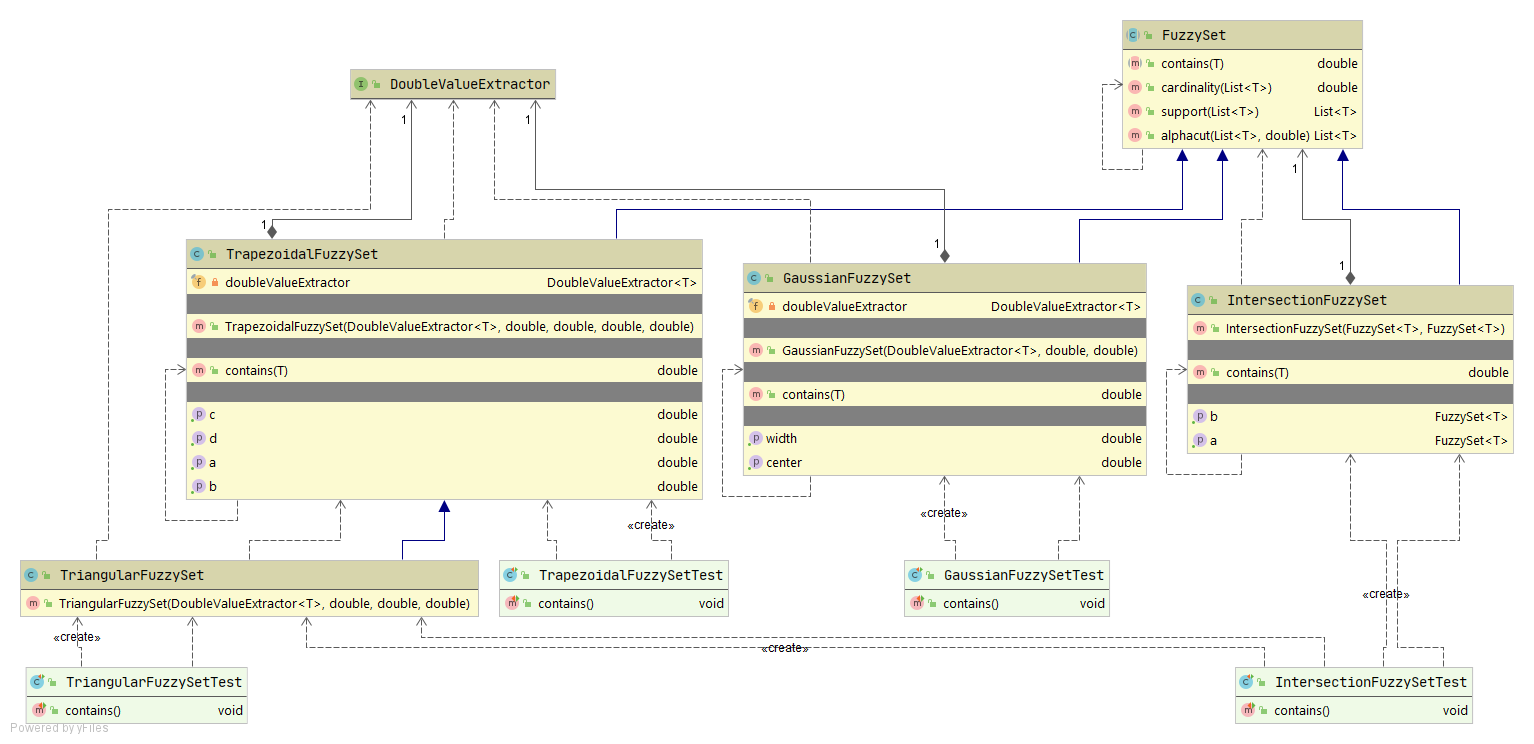
\includegraphics[width=\textwidth]{img/uml/logic_fuzzy_set.png}
                \caption{Diagram UML podpakietu \emph{set} biblioteki do obliczeń rozmytych}
            \end{figure}
            \FloatBarrier
            \begin{figure}[!htbp]
                \centering
                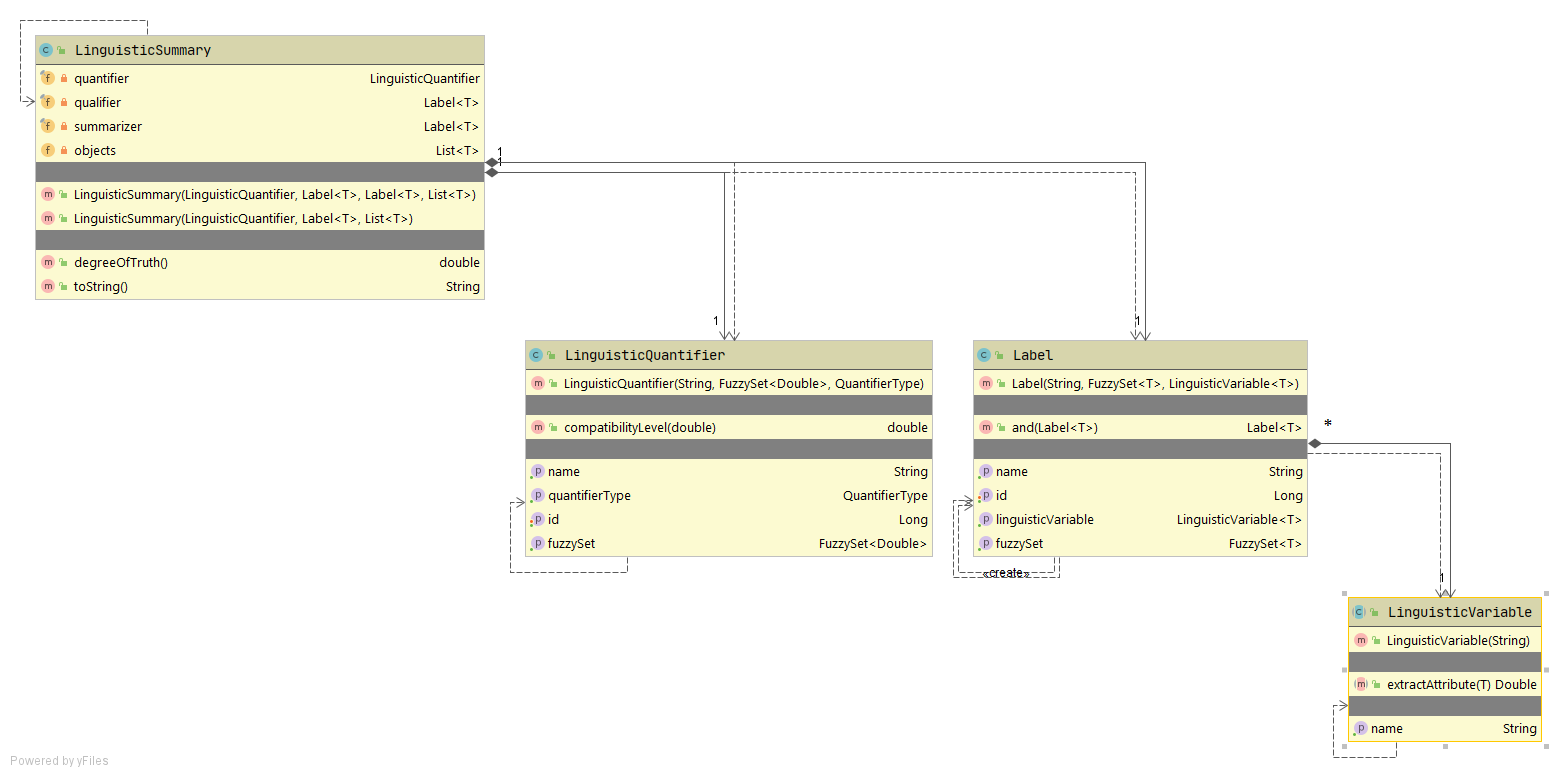
\includegraphics[width=0.7\textwidth]{img/uml/logic_fuzzy_linguistic.png}
                \caption{Diagram UML podpakietu \emph{linguistic} biblioteki do obliczeń rozmytych}
            \end{figure}
            \FloatBarrier
        }

        \subsection{Pakiet view} {
            Pakiet zawiera warstwę interfejsu graficzne użytkownika. W klasach i metodach zostały
            wykorzystane metody zaimplementowane w pakiecie logic. Dokładny podział na podpakiety
            został przedstawiony poniżej.
            \begin{description}
                \item[Pakiet \emph{constant}] zawiera stałe wykorzystywane w interfejsie użytkownka
                \item[Pakiet \emph{controller}] zawiera klasy kontrolerów odpowiedzialny za działanie poszczególnych okien
                \item[Pakiet \emph{fxml}] zawiera klasy zarządzające działaniem okien interfejsu użytkownika
                oraz klasy pomocnicze dla pakietu controller
            \end{description}
            \begin{figure}[!htbp]
                \centering
                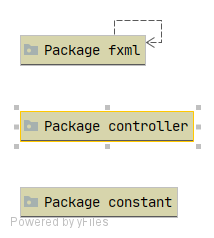
\includegraphics[width=0.3\textwidth]{img/uml/view.png}
                \caption{Diagram UML}
            \end{figure}
            \FloatBarrier
            Co wiecej poniżej zostały przedstawione poglądowe zrzuty ekranu interfejsu
            graficznego użytkownika
            \begin{figure}[!htbp]
            \centering
            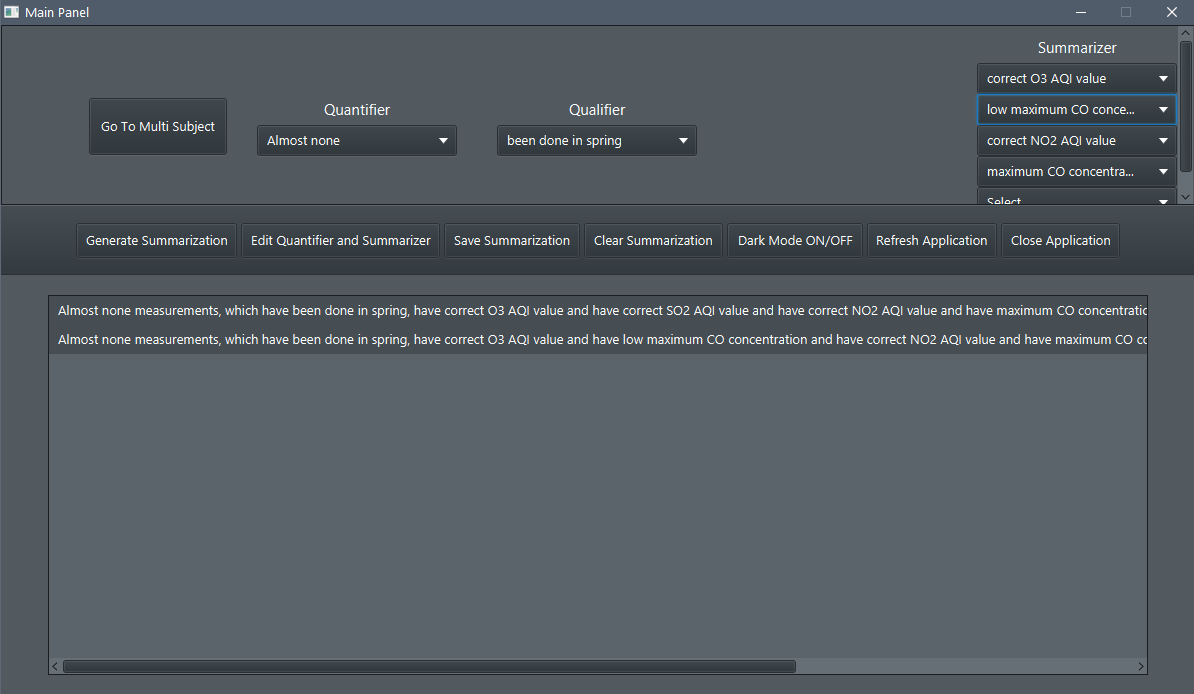
\includegraphics[width=1\textwidth]{img/gui/single_main.png}
            \caption{Panel głowny dla podsumowań jednopodmiotowych}
            \end{figure}
            \FloatBarrier

            \begin{figure}[!htbp]
            \centering
            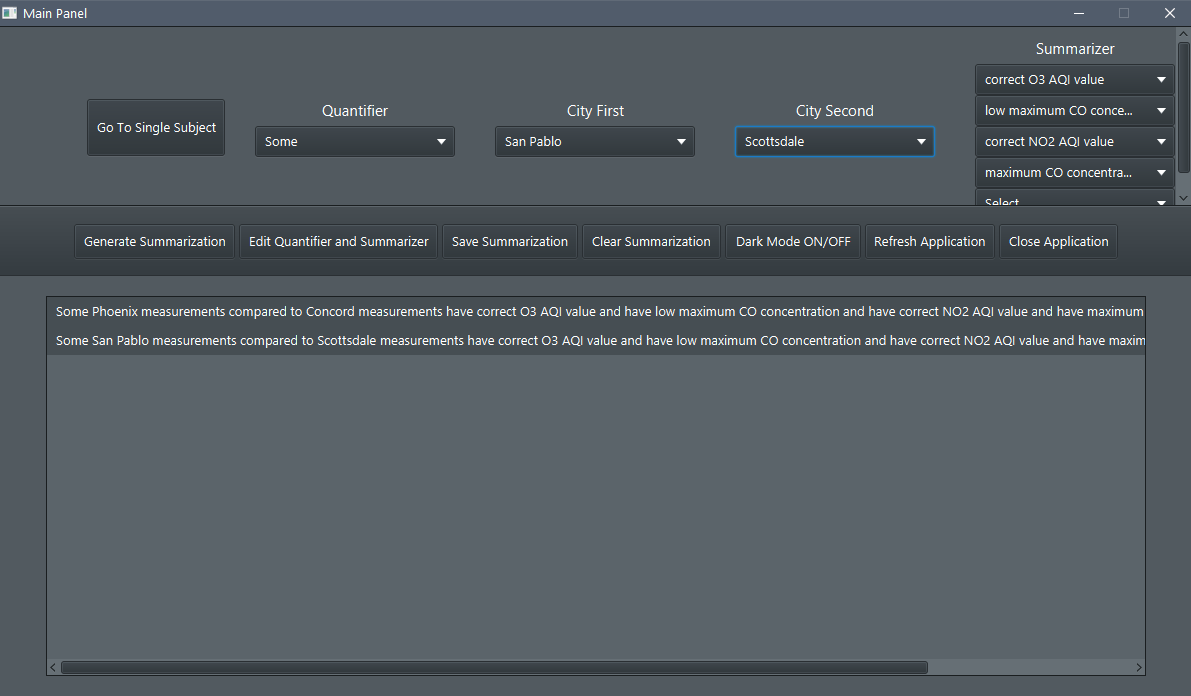
\includegraphics[width=1\textwidth]{img/gui/multi_main.png}
            \caption{Panel głowny dla podsumowań wielopodmiotowych}
            \end{figure}
            \FloatBarrier

            \begin{figure}[!htbp]
            \centering
            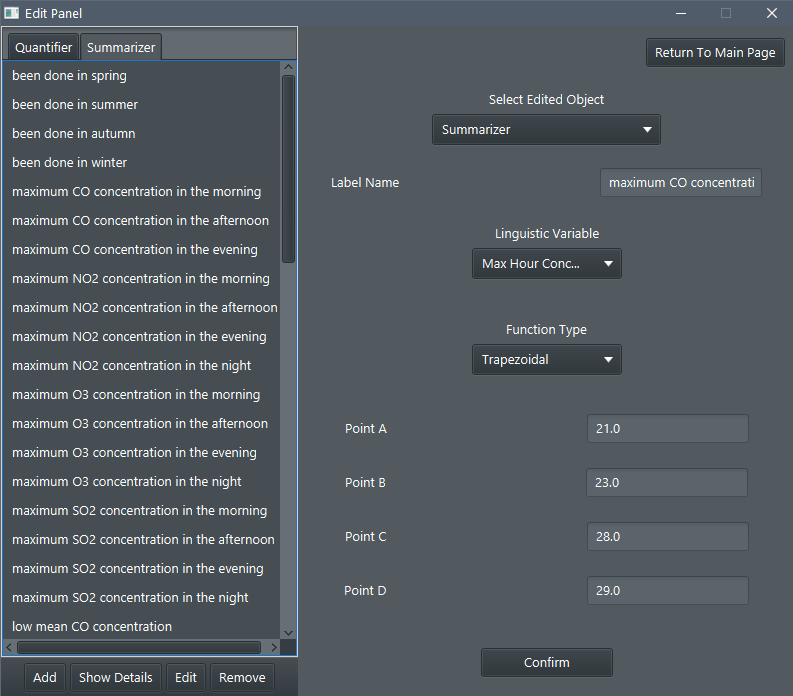
\includegraphics[width=0.8\textwidth]{img/gui/editor.png}
            \caption{Panel edycji dla użytkownika zaawansowanego}
            \end{figure}
            \FloatBarrier
        }

        \subsection{Pakiet mode} {
            Pakiet zawiera infrastrukturę programistyczną wspierającą rzetelne przeprowadzanie badań.
            Jego celem jest zapewnienie zarówno graficznego interfejsu użytkownika, jak i jego wersję
            konsolową. Wersja konsolowa charakteryzuje się tym, iż jest możliwość uruchamiania
            programu poprzez skrypt, w naszym przypadku jest to skrypt w języku Python. Co więcej,
            w skrypcie są przedstawione wszystkie zaplanowane eksperymenty. Skraca to czas wykonywania
            eksperymentów oraz eliminuje czynnik ludzki w ich przeprowadzaniu co za tym idzie ryzyko
            błednie przeprowadzonego eksperymentu diametralnie spada. Warto dodać, że tryb konsolowy
            jest dodatkowym trybem i wszystkie wymagania z instrukcji zostały spełnione, jest to
            jedynie nasz dodatek w celu usprawnienia procesu badań.

            \begin{description}
                \item[Klasa \emph{GraphicalMode}] odpowiada za uruchamianie i obsługę interfejsu użytkownika
                \item[Klasa \emph{CommandMode}] odpowiada za konsolowy tryb działania programu
            \end{description}
            \begin{figure}[!htbp]
                \centering
                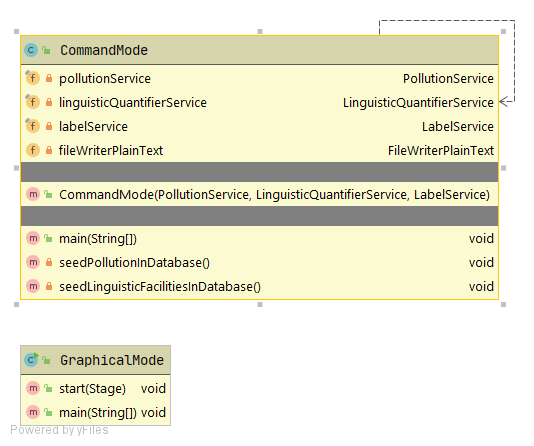
\includegraphics[width=0.5\textwidth]{img/uml/mode.png}
                \caption{Diagram UML}
            \end{figure}
            \FloatBarrier
        }
    }
    \newpage
%--------------------------------------------------------------------------------------%
    \section{Materiały i metody} {

        \subsection{Baza danych} {
            W programie i do późniejszych badań użyliśmy zbiór danych z pliku w formacie
            CSV~\cite{baza}, który został przekształcony na bazę danych. Zawiera ona dane
            dotyczące zanieczyszczeń powietrza w Stanach Zjednoczonych w latach 2000-2016.

            Aby zmiejszyć rozmiar bazy danych dokonano filtracji oryginalnego zbioru, poprzez
            usunięcie uznanych za zbędne kolumn o indeksach: 0 (identyfikator rekordu),
            1 - 3 (identyfikatory miejsca pomiaru, są zbędne, gdyż ta sama informacja jest
            przechowywana w innych kolumnach w postaci tekstowej) oraz 9, 14, 19, 24 (jednostki
            w których wyrażone są wartości liczbowe, zbędne gdyż zawsze takie same, dla całej
            kolumny). Usunięto także wszystkie rekordy, w których nie wszystkie atrybuty miały
            zdefiniowaną wartość.

            Po odfiltrowaniu baza składa się z 436876 rekordów, a każdy rekord posiada $21$
            atrybutów, w tym $17$ do rozmycia. Kolumny, nie zawierające wartości rozmywalnych
            opisują miejsce pomiaru i są to:
            \begin{enumerate}
                \item Adres
                \item Stan
                \item Hrabstwo
                \item Miasto
            \end{enumerate}

            \ \\
            Kolumny zawierające wartości do rozmycia to:
            \begin{enumerate}
                \item Data pomiaru - wartości z przedziału [2000-01-01 - 2016-05-31]
                \item Średnia stężenie danego tlenku - wartości z przedziału [-2 - 321.625]
                \item Maksymalna wartość w pomiarze danego tlenku - wartości z przedziału [-2 - 351]
                \item Godzine maksymalnego stężenia danego tlenku - wartości z przedziału [0 - 23]
                \item Indeks jakości powietrza (AQI) dla danego tlenku - wartości z przedziału [0 - 218]
            \end{enumerate}

            \ \\
            Pomiary zostały wykonane dla czterech różnych tlenków:
            \begin{enumerate}
                \item tlenek azotu(IV) $NO_2$  - jednostka ppb - liczba cząsteczek substancji na miliard cząsteczek powietrza
                \item tirtlen $O3$ - jednostka ppm - liczba cząsteczek substancji na milion cząsteczek powietrza
                \item tlenek siarki(IV) $SO2$ - jednostka ppb - liczba cząsteczek substancji na miliard cząsteczek powietrza
                \item tlenek węgla(II) $CO$ - jednostka ppm - liczba cząsteczek substancji na milion cząsteczek powietrza
            \end{enumerate}
        }

        \subsection{Zmienna lingwistyczne} {

            Poniżej zostały przedstawione zmienne lingwistyczne zaimplementowane w programie łącznie z dopasowanymi do nich
            etykietami. Wartym zaznaczenia jest fakt, że dla wszystkich tlenków zmienne lingwistyczne Max Hour Concentration
            zostały w sprawozdaniu przedstawione jako jedna zmienna lingwistyczna gdyż zbiory rozmyte etykiet tych zmiennych
            dla wszystkich tlenków są indentyczne. Kolejnym krokiem, którego celem jest zwiększenie czytelności sprawozdania
            i przedstawienie najbardziej znaczących fragmentów jest fakt, iż tylko dla tlenku siarki(IV) przedstawiliśmy
            wykresy funkcji przynależność dla wszystkich zmiennych lingwistycznych ww. tlenku.\\

            \begin{enumerate}
                \item Measurement Season
                \begin{itemize}
                    \item been done in spring
\begin{displaymath}
\mu_{been done in spring}(x) = \left\{ \begin{array}{ll}
0.02x + -0.53 & \textrm{dla $x \in [32, 92)$}\\
1 & \textrm{dla $x \in [92, 122)$}\\
-0.02x + 3.0 & \textrm{dla $x \in [122, 183]$}\\
\end{array} \right.
\end{displaymath}
                    \item been done in summer
\begin{displaymath}
\mu_{been done in summer}(x) = \left\{ \begin{array}{ll}
0.02x + -2.0 & \textrm{dla $x \in [122, 183)$}\\
1 & \textrm{dla $x \in [183, 214)$}\\
-0.02x + 4.51 & \textrm{dla $x \in [214, 275]$}\\
\end{array} \right.
\end{displaymath}
                    \item been done in autumn
\begin{displaymath}
\mu_{been done in autumn}(x) = \left\{ \begin{array}{ll}
0.02x + -3.51 & \textrm{dla $x \in [214, 275)$}\\
1 & \textrm{dla $x \in [275, 306)$}\\
-0.03x + 11.2 & \textrm{dla $x \in [306, 336]$}\\
\end{array} \right.
\end{displaymath}
                    \item been done in winter
\begin{displaymath}
\mu_{been done in winter}(x) = \left\{ \begin{array}{ll}
1 & \textrm{dla $x \in [0, 32)$}\\
-0.02x + 1.53 & \textrm{dla $x \in [32, 92)$}\\
0 & \textrm{dla $x \in [92, 275)$}\\
0.01x + -3.06 & \textrm{dla $x \in [275, 365]$}\\
\end{array} \right.
\end{displaymath}
                \end{itemize}
                \begin{figure}[!htbp]
                    \centering
                    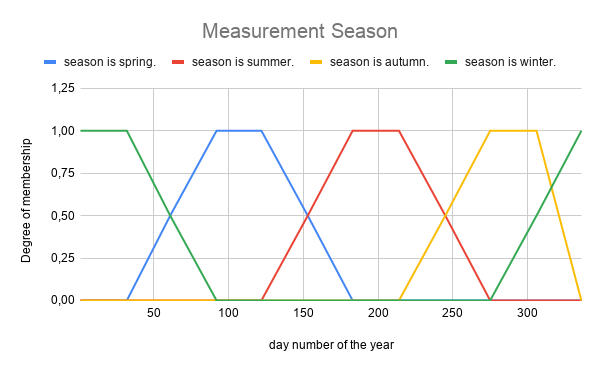
\includegraphics[width=0.9\textwidth]{img/theory/MeasurementSeason.png}
                    \caption{}
                \end{figure}
                \FloatBarrier
%--------------------------------------------------------------------------------------%
                \item Max Hour Concentration - dla wszystkich tlenków wzory funkcji przynależności są identyczne
                \begin{itemize}
                    \item maximum \emph{OXIDE NAME} concentration in the morning.
\begin{displaymath}
\mu_{maximum SO2 concentration in the morning}(x) = \left\{ \begin{array}{ll}
0.33x + -1.0 & \textrm{dla $x \in [3, 6)$}\\
1 & \textrm{dla $x \in [6, 10)$}\\
-0.33x + 4.33 & \textrm{dla $x \in [10, 13]$}\\
\end{array} \right.
\end{displaymath}
                    \item maximum \emph{OXIDE NAME} concentration in the afternoon.
\begin{displaymath}
\mu_{maximum SO2 concentration in the afternoon}(x) = \left\{ \begin{array}{ll}
1.0x + -12.0 & \textrm{dla $x \in [12, 13)$}\\
1 & \textrm{dla $x \in [13, 17)$}\\
-0.5x + 9.5 & \textrm{dla $x \in [17, 19]$}\\
\end{array} \right.
\end{displaymath}
                    \item maximum \emph{OXIDE NAME} concentration in the evening.
\begin{displaymath}
\mu_{maximum SO2 concentration in the evening}(x) = \left\{ \begin{array}{ll}
0.5x + -9.0 & \textrm{dla $x \in [18, 20)$}\\
1 & \textrm{dla $x \in [20, 21)$}\\
-1.0x + 22.0 & \textrm{dla $x \in [21, 22]$}\\
\end{array} \right.
\end{displaymath}
                    \item maximum \emph{OXIDE NAME} concentration in the night.
\begin{displaymath}
\mu_{maximum SO2 concentration in the night}(x) = \left\{ \begin{array}{ll}
1 & \textrm{dla $x \in [0, 4)$}\\
-1.0x + 5.0 & \textrm{dla $x \in [4, 5)$}\\
0 & \textrm{dla $x \in [5, 21)$}\\
0.5x + -10.5 & \textrm{dla $x \in [21, 23]$}\\
\end{array} \right.
\end{displaymath}
                \end{itemize}
                \begin{figure}[!htbp]
                    \centering
                    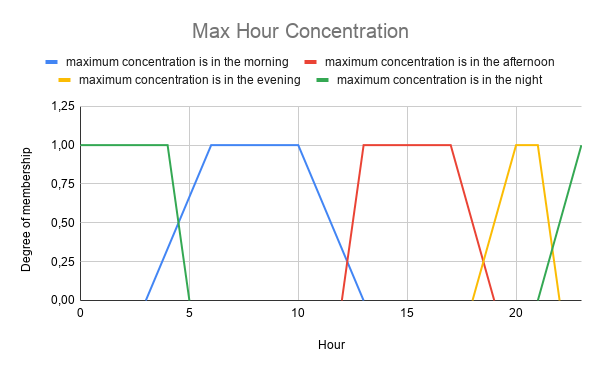
\includegraphics[width=0.9\textwidth]{img/theory/MaxHourConcentration.png}
                    \caption{}
                \end{figure}
                \FloatBarrier
%--------------------------------------------------------------------------------------%
                \item Mean Concentration CO
                \begin{itemize}
                    \item low mean CO concentration
                    \item middle mean CO concentration
                    \item high mean CO concentration
                \end{itemize}

                \item Mean Concentration NO2
                \begin{itemize}
                    \item low mean NO2 concentration
                    \item middle mean NO2 concentration
                    \item high mean NO2 concentration
                \end{itemize}

                \item Mean Concentration O3
                \begin{itemize}
                    \item low mean O3 concentration
                    \item middle mean O3 concentration
                    \item high mean O3 concentration
                \end{itemize}

                \item Mean Concentration SO2
                \begin{itemize}
                    \item low mean SO2 concentration
\begin{displaymath}
\mu_{low mean SO2 concentration}(x) = \left\{ \begin{array}{ll}
1 & \textrm{dla $x \in [0, 75)$}\\
-0.0x + 1.33 & \textrm{dla $x \in [75, 300]$}\\
\end{array} \right.
\end{displaymath}
                    \item middle mean SO2 concentration
\begin{displaymath}
\mu_{middle mean SO2 concentration}(x) = \left\{ \begin{array}{ll}
0.0x + -0.5 & \textrm{dla $x \in [150, 450)$}\\
1 & \textrm{dla $x \in [450, 600)$}\\
-0.01x + 4.0 & \textrm{dla $x \in [600, 800]$}\\
\end{array} \right.
\end{displaymath}
                    \item high mean SO2 concentration
\begin{displaymath}
\mu_{high mean SO2 concentration}(x) = \left\{ \begin{array}{ll}
0.0x + -1.5 & \textrm{dla $x \in [600, 1000]$}\\
\end{array} \right.
\end{displaymath}
                \end{itemize}
                \begin{figure}[!htbp]
                    \centering
                    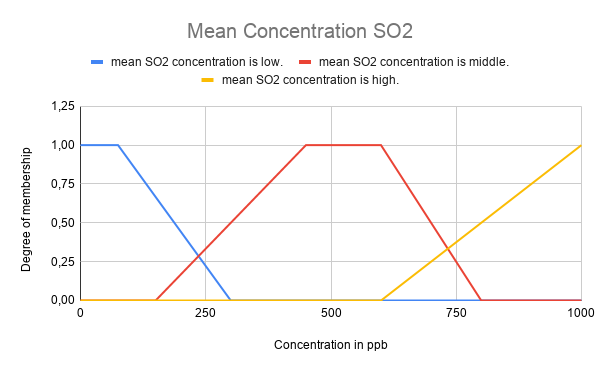
\includegraphics[width=0.9\textwidth]{img/theory/MeanConcentrationSO2.png}
                    \caption{}
                \end{figure}
                \FloatBarrier
%--------------------------------------------------------------------------------------%
                \item Max Concentration CO
                \begin{itemize}
                    \item low maximum CO concentration
                    \item middle maximum CO concentration
                    \item high maximum CO concentration
                \end{itemize}

                \item Max Concentration NO2
                \begin{itemize}
                    \item low maximum NO2 concentration
                    \item middle maximum NO2 concentration
                    \item high maximum NO2 concentration
                \end{itemize}

                \item Max Concentration O3
                \begin{itemize}
                    \item low maximum O3 concentration
                    \item middle maximum O3 concentration
                    \item high maximum O3 concentration
                \end{itemize}

                \item Max Concentration SO2
                \begin{itemize}
                    \item low maximum SO2 concentration
\begin{displaymath}
\mu_{low maximum SO2 concentration}(x) = \left\{ \begin{array}{ll}
1 & \textrm{dla $x \in [0, 75)$}\\
-0.0x + 1.33 & \textrm{dla $x \in [75, 300]$}\\
\end{array} \right.
\end{displaymath}
                    \item middle maximum SO2 concentration
\begin{displaymath}
\mu_{middle maximum SO2 concentration}(x) = \left\{ \begin{array}{ll}
0.0x + -0.5 & \textrm{dla $x \in [150, 450)$}\\
1 & \textrm{dla $x \in [450, 600)$}\\
-0.01x + 4.0 & \textrm{dla $x \in [600, 800]$}\\
\end{array} \right.
\end{displaymath}
                    \item high maximum SO2 concentration
\begin{displaymath}
\mu_{high maximum SO2 concentration}(x) = \left\{ \begin{array}{ll}
0.0x + -1.71 & \textrm{dla $x \in [600, 950)$}\\
1 & \textrm{dla $x \in [950, 1000]$}\\
\end{array} \right.
\end{displaymath}
                \end{itemize}
                \begin{figure}[!htbp]
                    \centering
                    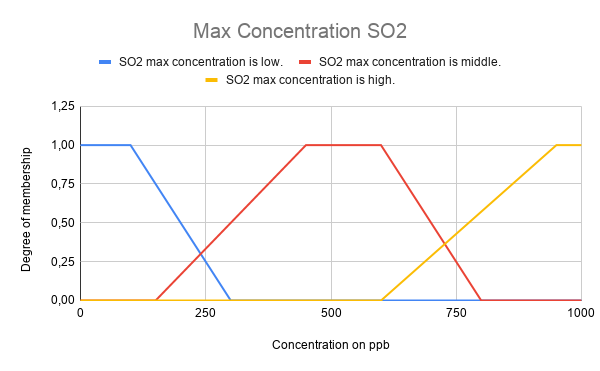
\includegraphics[width=0.9\textwidth]{img/theory/MaxConcentrationSO2.png}
                    \caption{}
                \end{figure}
                \FloatBarrier
%--------------------------------------------------------------------------------------%
                \item AQI Value CO
                \begin{itemize}
                    \item correct CO AQI value
                    \item unhealthy CO AQI value
                    \item hazardous CO AQI value
                \end{itemize}

                \item AQI Value NO2
                \begin{itemize}
                    \item correct NO2 AQI value
                    \item unhealthy NO2 AQI value
                    \item hazardous NO2 AQI value
                \end{itemize}

                \item AQI Value O3
                \begin{itemize}
                    \item correct O3 AQI value
                    \item unhealthy O3 AQI value
                    \item hazardous O3 AQI value
                \end{itemize}

                \item AQI Value SO2
                \begin{itemize}
                    \item correct SO2 AQI value
\begin{displaymath}
\mu_{correct SO2 AQI value}(x) = \left\{ \begin{array}{ll}
1 & \textrm{dla $x \in [0, 50)$}\\
-0.04x + 3.0 & \textrm{dla $x \in [50, 75]$}\\
\end{array} \right.
\end{displaymath}
                    \item unhealthy SO2 AQI value
\begin{displaymath}
\mu_{unhealthy SO2 AQI value}(x) = \left\{ \begin{array}{ll}
0.04x + -2.0 & \textrm{dla $x \in [50, 75)$}\\
1 & \textrm{dla $x \in [75, 150)$}\\
-0.01x + 2.5 & \textrm{dla $x \in [150, 250]$}\\
\end{array} \right.
\end{displaymath}
                    \item hazardous SO2 AQI value
\begin{displaymath}
\mu_{hazardous SO2 AQI value}(x) = \left\{ \begin{array}{ll}
0.01x + -1.5 & \textrm{dla $x \in [150, 250)$}\\
1 & \textrm{dla $x \in [250, 500]$}\\
\end{array} \right.
\end{displaymath}
                \end{itemize}
                \begin{figure}[!htbp]
                    \centering
                    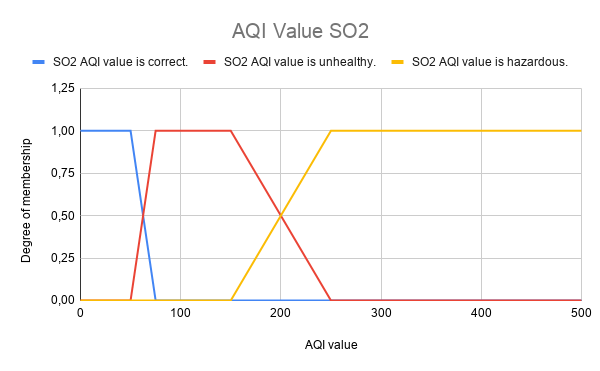
\includegraphics[width=0.9\textwidth]{img/theory/AQIValueSO2.png}
                    \caption{}
                \end{figure}
                \FloatBarrier
            \end{enumerate}
        }

        \subsection{Kwantyfikatory} {
            W programie zostały zastosowane poniższe kwantyfikatory
            \begin{itemize}
                \item Almost none
                \item Some
                \item About half of all
                \item Many
                \item All
            \end{itemize}

            \begin{figure}[!htbp]
                \centering
                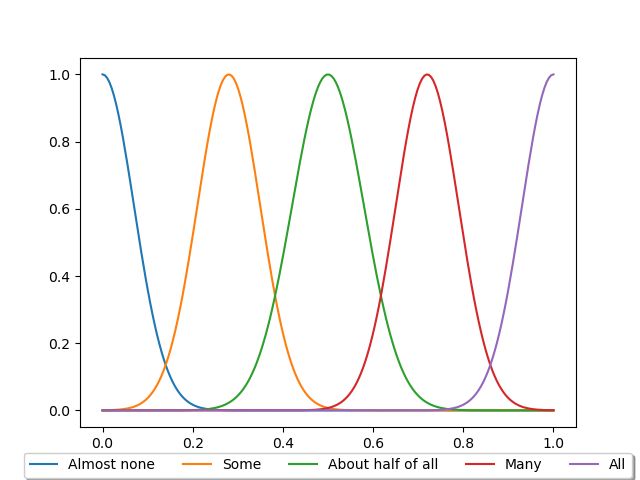
\includegraphics[width=0.7\textwidth]{img/theory/Quantifier.png}
                \caption{}
            \end{figure}
            \FloatBarrier
        }

        \subsection{Podsumowania lingwistyczne jednopodmiotowe w pierwszej formie} \label{jednopodmiot} {
            Wykorzystując wszystkie kombinacje opisanych wcześniej kwantyfikatorów (jest ich 5) oraz
            sumaryzatorów - etykiet (jest ich 56) wygenerowane zostały podsumowania w pierwszej
            formie z jednym sumaryzatorem. Wszystkich podsumowań jest oczywiście $5 \cdot 56 = 280$
            natomiast zanotowane w wynikach zostały tylke te, których jakość jest największa i które
            niosą najciekawsze informacje na temat zbioru danych. Po treści każdego z podsumowań
            wypisana została wartość ogólnej miary jakości, gdzie wagi dla kolejnych miar dobrane
            zostały w następujący sposób: $w_1 = 0.4$, $w_2 = 0.075$, $w_3 = 0.075$, $w_4 = 0.075$,
            $w_5 = 0.075$, $w_6 = 0$, $w_7 = 0$, $w_8 = 0.075$, $w_9 = 0.075$, $w_{10} = 0.075$,
            $w_{11} = 0.075$. Miary T6 i T7 nie zostały wzięte pod uwagę, ponieważ ze względu na
            kształt funkcji przynależności zbioru rozmytego kwantyfikatora (funkcja gaussa), wartość
            tych miar jest zawsze równa $0$. Ponadto spośród miar wziętych pod uwagę wyróżniona
            została miara T1 - uznaliśmy ją za najbardziej istotną dla oceny jakości podsumowania.
        }

        \subsection{Podsumowania lingwistyczne jednopodmiotowe w drugiej formie} {
            Postępując analogicznie do \ref{jednopodmiot} zostały wybrane jedynie podsumowania,
            które mają odpowiednio dużą wartość miary jakości i są najciekawsze pod względem
            możliwości oceny zawartości bazy danych.  Ponadto zotały one pogrupowane po
            kwantyfikatorze, dla lepszej czytelnościwyników. Co do liczby kombinacji jest to bardzo
            trudne do określenia gdyż kwantyfikatorów w programie mamy 5 sztuk, kwalifikatorów jest
            56 sztuk oraz summaryzatorów również jest 56 sztuk natomiast podsumowanie może się
            składać z dokładnie jednego kwantyfikatora, dokładnie jednego kwalifikatora oraz
            nieokreślonej, wiekszej lub równej jeden, liczbie summaryzatorów.  W wynikach
            wygenerowaliśmy oraz przedstawiliśmy podsumowania w wariantach:
            \begin{itemize}
                \item 1 kwantyfikator + 1 kwalifikator + 1 summaryzator
                \item 1 kwantyfikator + 1 kwalifikator + 2 summaryzator
            \end{itemize}
            Podobnie jak w poprzedniej serii wyników, tutaj również dla każdego podsumowania
            przedstawiona została wartość średniej ważonej wielu miar jakości.
        }

        \subsection{Podsumowania lingwistyczne wielopodmiotowe} {
            Kolejna seria podsumowań zawiera już podsumowania wielopodmiotowe, gdzie różne podmioty
            zostały uzyskane poprzez wyodrębnienia z głównego zbioru danych par podzbiorów według
            kryterium, którym jest miasto, gdzie dokonano pomiaru. Wykorzystano miasta: Los Angeles,
            New York, Phoenix i El Paso. Tak wyodrębnione podmioty wykorzystane zostały do
            wygenerowani niewielkiej liczby przykładowych podsumowań wielopodmiotowych w pierwszej,
            drugiej i trzeciej formie, dla których jedyną miarą jakości, której wartość obliczono
            jest T1 - poziom prawdziwości.  Wartość wspomnianej miary jakości jest również
            podstawowym kryterium, na podstawie którego spośród wielu różnych możliwych podsumowań
            wyselekcjonowano te, które warto było tutaj przedstawić.
        }

    }
%--------------------------------------------------------------------------------------%
    \section{Wyniki} {
        \subsection{Podsumowania lingwistyczne jednopodmiotowe w pierwszej formie} {
            \begin{enumerate}
                \item About half of all measurements have maximum SO2 concentration in the morning. [0.41]
                \item Almost none measurements have hazardous CO AQI value. [0.70]
                \item Almost none measurements have hazardous NO2 AQI value. [0.70]
                \item Almost none measurements have maximum CO concentration in the afternoon. [0.64]
                \item Almost none measurements have maximum CO concentration in the evening. [0.63]
                \item Almost none measurements have maximum NO2 concentration in the afternoon. [0.45]
                \item Almost none measurements have maximum O3 concentration in the afternoon. [0.58]
                \item Almost none measurements have maximum O3 concentration in the evening. [0.67]
                \item Almost none measurements have maximum O3 concentration in the night. [0.49]
                \item Almost none measurements have maximum SO2 concentration in the evening. [0.56]
                \item Almost none measurements have unhealthy CO AQI value. [0.70]
                \item Almost none measurements have unhealthy O3 AQI value. [0.53]
                \item Many measurements have correct NO2 AQI value. [0.65]
                \item Many measurements have maximum CO concentration in the night. [0.43]
                \item Many measurements have maximum O3 concentration in the morning. [0.65]
                \item Some measurements have been done in summer. [0.68]
                \item Some measurements have been done in winter. [0.67]
                \item Some measurements have correct CO AQI value. [0.60]
                \item Some measurements have correct SO2 AQI value. [0.59]
                \item Some measurements have maximum CO concentration in the morning. [0.64]
                \item Some measurements have maximum NO2 concentration in the evening. [0.43]
                \item Some measurements have maximum NO2 concentration in the morning. [0.57]
                \item Some measurements have maximum NO2 concentration in the night. [0.68]
                \item Some measurements have maximum SO2 concentration in the night. [0.58]
            \end{enumerate}
        }

        \subsection{Podsumowania lingwistyczne jednopodmiotowe w drugiej formie} {
            \begin{enumerate}
                \item About half of all measurements, which have been done in winter, have correct CO AQI value. [0.57]
                \item About half of all measurements, which have maximum CO concentration in the evening, have unhealthy CO AQI value. [0.44]
                \item About half of all measurements, which have maximum NO2 concentration in the afternoon, have been done in winter and have correct NO2 AQI value. [0.79]
                \item About half of all measurements, which have maximum O3 concentration in the evening, have been done in winter and have correct O3 AQI value. [0.72]
                \item About half of all measurements, which have maximum O3 concentration in the night, have been done in winter and have correct O3 AQI value. [0.65]
                \item All measurements, which have been done in autumn, have correct O3 AQI value. [0.48]
                \item All measurements, which have been done in spring, have correct O3 AQI value. [0.57]
                \item All measurements, which have maximum NO2 concentration in the afternoon, have been done in winter and have correct NO2 AQI value. [0.42]
                \item All measurements, which have maximum O3 concentration in the evening, have been done in winter and have correct O3 AQI value. [0.42]
                \item All measurements, which have maximum O3 concentration in the evening, have correct O3 AQI value. [0.52]
                \item Almost none measurements, which have been done in autumn, have unhealthy O3 AQI value. [0.69]
                \item Almost none measurements, which have maximum NO2 concentration in the afternoon, have been done in winter and have unhealthy NO2 AQI value. [0.78]
                \item Almost none measurements, which have maximum O3 concentration in the afternoon, have been done in spring and have unhealthy O3 AQI value. [0.79]
                \item Almost none measurements, which have maximum SO2 concentration in the evening, have been done in autumn and have correct SO2 AQI value. [0.62]
                \item Many measurements, which have been done in spring, have correct NO2 AQI value. [0.64]
                \item Many measurements, which have been done in summer, have correct NO2 AQI value. [0.73]
                \item Many measurements, which have maximum NO2 concentration in the afternoon, have correct NO2 AQI value. [0.77]
                \item Many measurements, which have maximum NO2 concentration in the morning, have correct NO2 AQI value. [0.73]
                \item Many measurements, which have maximum NO2 concentration in the night, have correct NO2 AQI value. [0.75]
                \item Many measurements, which have maximum O3 concentration in the evening, have been done in winter and have correct O3 AQI value. [0.42]
                \item Many measurements, which have maximum O3 concentration in the night, have been done in winter and have correct O3 AQI value. [0.42]
                \item Some measurements, which have been done in spring, have correct CO AQI value. [0.78]
                \item Some measurements, which have maximum NO2 concentration in the afternoon, have been done in autumn and have correct NO2 AQI value. [0.73]
                \item Some measurements, which have maximum O3 concentration in the afternoon, have been done in spring and have correct O3 AQI value. [0.76]
                \item Some measurements, which have maximum SO2 concentration in the afternoon, have correct SO2 AQI value. [0.81]
                \item Some measurements, which have maximum SO2 concentration in the evening, have correct SO2 AQI value. [0.82]
            \end{enumerate}
        }

        \subsection{Podsumowania lingwistyczne wielopodmiotowe w pierwszej formie} {
            \begin{enumerate}
                \item About half of all Los Angeles measurements compared to El Paso measurements have correct NO2 AQI value. [0.99]
                \item About half of all Los Angeles measurements compared to Phoenix measurements have unhealthy SO2 AQI value. [0.82]
                \item About half of all New York measurements compared to Los Angeles measurements have maximum O3 concentration in the morning. [0.87]
                \item About half of all New York measurements compared to Phoenix measurements have maximum CO concentration in the morning. [0.94]
                \item About half of all New York measurements compared to Phoenix measurements have maximum NO2 concentration in the night. [0.99]
                \item About half of all Phoenix measurements compared to El Paso measurements have correct NO2 AQI value. [0.98]
                \item About half of all Phoenix measurements compared to El Paso measurements have maximum CO concentration in the night. [0.96]
                \item All Los Angeles measurements compared to El Paso measurements have unhealthy CO AQI value. [0.61]
                \item Almost none New York measurements compared to Los Angeles measurements have unhealthy CO AQI value. [0.87]
                \item Many Los Angeles measurements compared to Phoenix measurements have maximum CO concentration in the afternoon. [1.00]
                \item Many Los Angeles measurements compared to Phoenix measurements have maximum O3 concentration in the afternoon. [0.91]
                \item Many Los Angeles measurements compared to Phoenix measurements have unhealthy CO AQI value. [0.99]
                \item Many New York measurements compared to El Paso measurements have maximum O3 concentration in the evening. [0.99]
                \item Many New York measurements compared to Phoenix measurements have correct SO2 AQI value. [0.98]
                \item Some Los Angeles measurements compared to Phoenix measurements have maximum SO2 concentration in the evening. [0.86]
                \item Some New York measurements compared to Los Angeles measurements have unhealthy NO2 AQI value. [0.84]
                \item Some New York measurements compared to Phoenix measurements have unhealthy O3 AQI value. [0.99]
                \item Some Phoenix measurements compared to El Paso measurements have maximum SO2 concentration in the afternoon. [0.92]
            \end{enumerate}
        }
        
        \subsection{Podsumowania lingwistyczne wielopodmiotowe w drugiej formie} {
            \begin{enumerate}
                \item About half of all Los Angeles measurements compared to El Paso measurements, which have maximum O3 concentration in the morning, have correct O3 AQI value. [0.90]
                \item About half of all New York measurements compared to El Paso measurements, which have maximum O3 concentration in the morning, have correct O3 AQI value. [0.99]
                \item About half of all New York measurements compared to Los Angeles measurements, which have maximum NO2 concentration in the morning, have unhealthy NO2 AQI value. [0.77]
                \item All Los Angeles measurements compared to El Paso measurements, which have maximum O3 concentration in the night, have unhealthy O3 AQI value. [1.00]
                \item All Los Angeles measurements compared to Phoenix measurements, which have maximum CO concentration in the morning, have unhealthy CO AQI value. [0.77]
                \item All Los Angeles measurements compared to Phoenix measurements, which have maximum O3 concentration in the evening, have correct O3 AQI value. [0.99]
                \item Many Los Angeles measurements compared to El Paso measurements, which have maximum NO2 concentration in the night, have correct NO2 AQI value. [0.53]
                \item Many Los Angeles measurements compared to Phoenix measurements, which have maximum SO2 concentration in the morning, have correct SO2 AQI value. [0.68]
                \item Many New York measurements compared to Phoenix measurements, which have maximum NO2 concentration in the night, have correct NO2 AQI value. [0.82]
                \item Many Phoenix measurements compared to El Paso measurements, which have maximum SO2 concentration in the evening, have unhealthy SO2 AQI value. [1.00]
                \item Some Los Angeles measurements compared to Phoenix measurements, which have maximum O3 concentration in the morning, have unhealthy O3 AQI value. [0.86]
                \item Some New York measurements compared to El Paso measurements, which have maximum CO concentration in the night, have unhealthy CO AQI value. [0.74]
                \item Some New York measurements compared to Phoenix measurements, which have maximum O3 concentration in the morning, have unhealthy O3 AQI value. [0.80]
            \end{enumerate}
        }

        \subsection{Podsumowania lingwistyczne wielopodmiotowe w trzeciej formie} {
            \begin{enumerate}
                \item About half of all Los Angeles measurements, which have maximum CO concentration in the morning, compared to El Paso measurements have correct CO AQI value. [0.82]
                \item About half of all New York measurements, which have maximum NO2 concentration in the evening, compared to El Paso measurements have unhealthy NO2 AQI value. [0.82]
                \item About half of all Phoenix measurements, which have maximum O3 concentration in the morning, compared to El Paso measurements have correct O3 AQI value. [0.78]
                \item All New York measurements, which have maximum SO2 concentration in the morning, compared to El Paso measurements have hazardous SO2 AQI value. [1.00]
                \item All New York measurements, which have maximum SO2 concentration in the morning, compared to El Paso measurements have unhealthy SO2 AQI value. [0.98]
                \item All New York measurements, which have maximum SO2 concentration in the morning, compared to Los Angeles measurements have hazardous SO2 AQI value. [1.00]
                \item Almost none Los Angeles measurements, which have maximum CO concentration in the afternoon, compared to El Paso measurements have unhealthy CO AQI value. [1.00]
                \item Almost none Los Angeles measurements, which have maximum O3 concentration in the afternoon, compared to El Paso measurements have unhealthy O3 AQI value. [0.97]
                \item Almost none Los Angeles measurements, which have maximum O3 concentration in the evening, compared to Phoenix measurements have correct O3 AQI value. [0.99]
                \item Many Los Angeles measurements, which have maximum CO concentration in the morning, compared to El Paso measurements have unhealthy CO AQI value. [0.96]
                \item Many New York measurements, which have maximum SO2 concentration in the morning, compared to El Paso measurements have correct SO2 AQI value. [1.00]
                \item Many New York measurements, which have maximum SO2 concentration in the morning, compared to Los Angeles measurements have correct SO2 AQI value. [0.42]
                \item Some Los Angeles measurements, which have maximum CO concentration in the morning, compared to Phoenix measurements have correct CO AQI value. [0.90]
                \item Some Los Angeles measurements, which have maximum O3 concentration in the morning, compared to Phoenix measurements have unhealthy O3 AQI value. [0.95]
                \item Some New York measurements, which have maximum CO concentration in the morning, compared to El Paso measurements have correct CO AQI value. [0.87]
            \end{enumerate}
        }
    }
%--------------------------------------------------------------------------------------%
    \section{Dyskusja} {
        Pierwsza seria wyników dotyczy podsumowań lingwistycznych jednopodmiotowych w pierwszej
        formie - oznacza to oczywiście, że nie występuje tutaj kwalifikator. Podczas liczenia
        jakości podsumowania, punktem odniesienia dla liczby pomiarów posiadających wybraną cechę są
        wszystkie pomiary. Wybrane zostały te podsumowania, które niosą najwięcej informacji i mają
        najwyższą jakość - są najbardziej prawdziwe i precyzyjne. Warto zauważyć, że niektóre z
        podsumowań niosą informacje bardzo cenne i konkretne, inne natomiast prowadzą do wniosków
        zupełnie oczywistych. Pierwsze dwa podsumowania "Some measurements have been done in
        summer/winter" oznaczają oczywiście, że po prostu jakaś część (zapewne ok 25\%) podsumowań,
        była zrobiona w danej porze roku - wniosek jest więc taki, że pomiary były robione
        równomiernie przez cały rok. Nie jest to informacja szczególnie odkrywcza, ale konkretna.
        Podobne wnioski na temat rozkładu wartości danych pomiarowych niosą inne podsumowania z
        kwantyfikatorem \emph{some}, których jest tutaj całkiem sporo, jako że dla tego
        kwantyfikatora łatwiej jest uzyskać wysoki poziom prawdziwości niż dla np. \emph{all} lub
        \emph{many} - przy rozkładzie normalnym zawsze znajdzie się przynajmniej kilka obiektów
        posiadających daną cechę. Tak więc pojawiają się jeszcze podsumowania typu "Some
        measurements have correct CO/SO2 AQI value", lub "Some measurements have maximum SO2/NO2/CO
        concetration in the evening/morning". Wszystko to pozwala wywnioskować, że wspomniane
        wartości parametrów (sumaryzatorów) czasami zdarzają się w zbiorze danych. Podobnie sytuacja
        ma się z kwantyfikatorem \emph{almost none}, który pojawia się chyba w największej grupie
        uzyskanych podsumowań jednopodmiotowych. Te wyniki pozwalają dotrzec, które cechy rzadko
        albo prawie nigdy nie występują w zbiorze danych. Można do nich tutaj zaliczyć "maximum
        CO/O3 concetration in the evening", czy "hazardous AQI" i "unhealthy AQI". Te dwa ostatnie
        prowadzą do ciekawych wniosków, że stosunkowo rzadko w ogóle zanieczyszczenie powietrza w
        badanych rejonach jest naprawdę wysokie lub groźne. Okazuje się również, że tlenki CO i O3
        nie mają zazwyczaj najwyższego stężenia w godzinach wieczornych. Jak widać kwantyfikator ten
        pozwala otrzymać dosyć precyzyjne podsumowania, niosące wiele informacji. Ostatecznie jednak
        łatwiej znaleźć cechę której obiekt nie ma, niż którą obiekt ma i dlatego najcenniejsze oraz
        jednocześnie trudniejsze do znalezienia są wyrażenia z kwantyfikatorem \emph{many} lub
        \emph{all}. W przypadku omawianej pierwszej grupy podsumowań dobrym przykładem jest "Many
        measurements have maximum O3 concentration in the morning.". Mamy tutaj zawartą konkretną i
        nie zostawiającą miejsca do interpretacji informację - największe zanieczyszczenie
        tritlenkiem występuje z rana. Innym przykładem jest "Many measurements have correct NO2 AQI
        value." - zazwyczaj średnie stężenie NO2 jest całkiem normalne i bezpieczne.

        Opisane powyże podsumowania jenopodmiotowe zawierają informacje ogólne, dotyczące całego
        zbioru danych. Są one bardzo cenne i łatwe w interpretacji, jednak nie można wysnuć na ich
        podstawie żadnych wniosków, dotyczących pewnych wybranych podzbiorów wszystkich pomiarów.
        Informacje takie mogłyby okazać się również bardzo cenne, ze względu na swój bardziej
        szczegółowych charakter. Druga seria wyników dotyczy właśnie podsumowań jednopodmiotowych w
        drugiej formie, które to uzupełniają wspomniane braki podsumowań w formie pierwszej. Dla
        przejrzystości wyników zostały one pogrupowane według kwantyfikatorów, które, jak opisano
        powyżej, mają kluczowe znaczenie dla praktycznej wartości wygenerowanego podsumowania.
        Pierwsza grupa wyników jest oparta o kwantyfikator \emph{all}. Te podsumowania wyróżniają
        podgrupy pomiarów, które w zdecydowanej większości posiadają pewną szczególną cechę. I tak
        np. "All measurements, which have maximum O3 concentration in the evening, have been done in
        winter and have correct O3 AQI value." oznacza, że dni, kiedy najwyższe stężenie tritlenku
        jest wieczorem, praktycznie zdarzają się tylko zimą. Podobnie "All measurements, which have
        been done in spring, have correct O3 AQI value." prowadzi do wniosków, że wskaźnik AQI dla
        tritlenku jest zawsze poprawny wiosną. Istnieje jednak ryzyko, że cechy wskazane tutaj jako
        charakterystyczne dla pewnych podzbiorów, mogą być również prawdziwe dla całego podzbioru,
        co czynik takie podsumowania mało wartościowymi. Kolejny kwantyfikator to \emph{many}. Te
        podsumowania wydają się najciekawsze. Pozwalają wysnuć wnioski, że zimą zanieczyszczenia
        osiągają najwyższy poziom raczej wieczorem, niż z rana.  Ciekawym podsumowaniem jest również
        "Many measurements, which have maximum NO2 concentration in the morning, have correct NO2
        AQI value.", które pozwala zauważyć, że jeżeli stężenie NO2 jest najwyższe w godzinach
        porannych, znaczy to, że zanieczyszczenie nie jest zbyt duże.  Warto jeszcze wspomnieć o
        "Many measurements, which have been done in spring, have correct NO2 AQI value.", gdzie
        okazuje się, że wiosną (ale również i latem jak stoi w innym podsumowaniu), stężenie NO2 nie
        jest za wysokie.  Można pokusić się o wniosek, że wiosną i latem w ogóle powietrze jest
        zdrowsze, nie jest to jednak wniosek pewny. Po podsumowaniach z kwantyfikatorem \emph{many}
        mamy do czynienia z podsumowaniami opartymi o \emph{about half of}. Przykładowe wyniki to:
        "About half of all measurements, which have maximum CO concentration in the evening, have
        unhealthy CO AQI value.", czy "About half of all measurements, which have maximum O3
        concentration in the night, have been done in winter and have correct O3 AQI value.".
        Pierwsze z tych dwóch ma zdecydowanie niższą jakość, ale również i wniosek jest bardziej
        "śmiały", gdyż podsumowani to pozwala stwierdzić, że całkiem często (niemalże w połowie
        przypadków), gdy stężenie CO jest najwyższe wieczorem, to średnie stężenie tego tlenku
        rówież jest za wysokie. Kolejne podsumowanie ma znacznie wyższą jakość i mówi znowu o tym,
        że często zimą najwyższe stężenie zanieczyzczeń jest nocą. Ostatnia dwie grupy podsumowań to
        te zawierające kwantyfikatory \emph{almost none} oraz \emph{some}. Jako, że te
        kwantyfikatory zostały najdokładniej omówione przy podsumowanich w formie pierwszej,
        przytoczymy jedynie kilka co ciekawszych przykładów. Mamy tutaj "Some measurements, which
        have been done in spring, have correct CO AQI value." oraz np.  "Almost none measurements,
        which have been done in autumn, have unhealthy O3 AQI value.". Pierwsze z nich, oznacza, że
        istnieje jakaś grupa pomiarów wykonanych wiosną, gdzie wskaźnik AQI dla CO ma wartość
        poprawną.  Drugie natomiast jest całkiem ciekawe i mówi o tym, że praktycznie nie zdzarza
        się, aby jesienią wskaźnik AQI dla tritlenku był niezdrowy.  Na podstawie dotychczas
        omówionych podsumowań można powoli zauważyć powne zależności w badanym zbiorze danych.
        Okazuje się, że najgorsza jest jakość powietrza zimą (co jest logiczne, bo ludzie
        się ogrzewają) i że zazwyczaj wtedy maksymalne stężenie zanieczyszczeń w powietrzu występują
        wieczorem lub w nocy. Podobnych wniosków nie można by otrzymać z podsumowań w formie
        pierwszej. Warto jescze zwrócić uwagę na jakości podsumowań, cała druga seria wyników
        potwierdza co było już powiedziane przy omawianiu pierwszej serii, że łatwiej jest znaleźć
        podsumowania o wysokim stopniu prawdziwości dla kwantyfikatorów \emph{some} czy \emph{almost
        none}. Widzimy, że faktycznie podsumowania z tymi kwantyfikatorami mają  lepszą jakość, niż
        te z pozostałymi kwantyfikatorami.

        Kolejna grupa wyników dotyczy podsumowań wielopodmiotowych w pierwszej formie. Miarą jakości
        nie jest tu już średnia ważona ale uwzględniony został jedynie poziom prawdziwości.
        Większość tych podsumowań jest bardzo ciekawa. Udało się wygenerować jedno podsumowanie z
        kwantyfikatorem \emph{all}: "All Los Angeles measurements compared to El Paso measurements
        have unhealthy CO AQI value.". Prowadzi ono do podobnych wniosków jak "Many Los Angeles
        measurements compared to Phoenix measurements have unhealthy CO AQI value.", a mianowicie,
        że generalnie powietrze w Los Angeles jest bardziej zanieczyszczone niż w Phoenix czy w El
        Paso. Trochę inne wyniki otrzymaliśmy dla New York: "Many New York measurements compared to
        El Paso measurements have maximum O3 concentration in the evening." oraz "Many New York
        measurements compared to Phoenix measurements have correct SO2 AQI value.", gdzie to drugie
        podsumowanie mówi o tym, że w New York jest dobra jakość wskaźnika AQI dla SO2 w porównianiu
        do miasta Phoenix. Dalej wygenerowane zostały podsumowania oparte o o kolejne
        kwantyfikatory, w tym np. "About half of all Los Angeles measurements compared to Phoenix
        measurements have unhealthy SO2 AQI value." potwierdzające niską jakość powietrza w Los
        Angeles. Niektóre podsumowania dotyczą porównania godzin maksymalnego stężenia w miastach:
        "Some Los Angeles measurements compared to Phoenix measurements have maximum SO2
        concentration in the evening.", "About half of all New York measurements compared to Los
        Angeles measurements have maximum O3 concentration in the morning.". Pozwalają one
        stwierdzić, że czasami wyższe stężenie zanieczyszczeń występuje w godzinach wieczornych w
        Los Angeles w porównianiu do Phoenix, oraz w godzinach porannych w New York, w porównaniu do
        Los Angeles. Łącząc tę informację z poprzednio uzyskanymi wnioskami na temat zależności
        między godziną maksymalnego stężenia a ogólnym stanem powietrza można pokusić się o kolejne
        potwierdzenie, że w Los Angeles zanieczyszczenie powietrza jest wysokie. Na końcu warto
        podkreślić, że uzyskane informacje dotyczące zależności między zanieczyszczeniem powietrza w
        różnych miastach były zupełnie niemożliwe do uzyskania z wykorzystaniem podsumowań
        jednopodmiotowych. Trzeba również zwrócić uwagę na fakt, że podsumowania wielopodmiotowe są
        cenniejsze, kiedy można uzyskane z nich informacje skonfrontować z tymi uzyskanymi z
        podsumowań jednopodmiotowych.

        Ostatnie dwie serie podsumowań są typu wielopodmiotowego w formie drugiej i trzeciej.
        Występuje więc tutaj kwalifikator, który raz dotyczy pierwszego a raz drugiego podmiotu.
        Podobnie jak w poprzednich eksperymentach również i tu można znaleźć ciekawe wyniki.
        Jednakże najważniejsze, na co trzeba zwrócić uwagę w przypadku tego rodzaju podsumowań to
        fakt, że jeżeli kwalifikator nie będzie "pokrywał" prawie żadnego elementu ze zbioru, to
        jakość podsumowań będzie wynikała ze stosunku dwóch zbiorów, gdzie jeden jest pusty a drugi
        nie. W ten sposób pojawi się bardzo dużo prawdziwych podsumowań, które nie niosą żadnej
        informacji. W przypadku podsumowań w drugiej formie, najwięcej prawdziwych podsumowań w
        stopniu prawie $1.0$ było związanych z kwalifikatorem \emph{all}. Zamieszczono tutaj tylko
        kilka przykładów, ale podczas testowania wielu kombinacji to zjawisko było łatwe do
        zaobserwowania. Podobnie w podsumowaniach typu trzeciego najwięcej prawdziwych było
        związanych z kwalifikatorem \emph{almost none}. Wynika to z faktu, że kwalifikator
        "eliminował" wszystkie elementy ze zbioru będącego podmiotem pierwszym i większość
        podsumowań, gdzie pierwszy podmiot nie posiadał jakiejś cechy w stosunku do podmiotu
        drugiego, okazywała się prawdziwa.
    }
%--------------------------------------------------------------------------------------%
    \section{Wnioski} {
        \begin{itemize}
            \item Podsumowania lingwistyczne, w zależności od wykorzystanych
                określeń, mogą nieść informacje bardzo cenne i odkrywcze lub
                zupełnie oczywiste i niezbyt wartościowe
            \item Podczas szukania jak najbardziej prawdziwych podsumowań,
                najłatwiej jest znaleźć to oparte o kwantyfikator \emph{some} i
                \emph{almost none}
            \item Podsumowania lingwistyczne w pierwszej formie zawierają
                informacje bardziej ogólne ale łatwiejsze do zrozumienia i
                zinterpretowania
            \item Podsumowania wielopodmiotowe mają bardziej szczegółowy charakter
                i pozwalają znaleźć bardziej subtelne cechy zbioru lub podzbiorów
                badanych obiektów, często niemożliwych do zauważenia na podstawie
                podsumowań jednopodmiotowych
            \item Podsumowania wielopodmiotowe, w przeciwieństwie do
                jednopodmiotowych, dają możliwość znalezienia pewnych zależności,
                między pewnymi grupami obiektów (podmiotami) w badanym zbiorze
                danych
            \item W podsumowaniach wielopodmiotowych, wykorzystując odpowiedni
                kwalifikator i kwantyfikator, łatwo można otrzymać wysoki poziom
                prawdziwości dla podsumowań nie wnoszących praktycznie żadnych
                informacji
            \item Podsumowania różnych typów uzupełniają się wzajemnie
            \item Powietrze w USA nie jest w takim tragicznym stanie (są
                wyjątki, jak Los Angeles)
        \end{itemize}
    }
%--------------------------------------------------------------------------------------%
    \begin{thebibliography}{0}
        \bibitem{an2008}{Niewiadomski, Adam. Methods for the Linguistic Summarization of Data: Applications of Fuzzy Sets and Their Extensions. Akademicka Oficyna Wydawnicza EXIT, Warszawa 2008. ISBN: 978-83-60434-40-6}
        \bibitem{an2019}{Niewiadomski, Adam. Zbiory rozmyte typu 2. Zastosowania w reprezentacji informacji. Akademicka Oficyna Wydawnicza EXIT, 2019. ISBN: 978-83-7837-595-1}
        \bibitem{baza}{Kaggle. U.S. Pollution Data[online]. [dostęp 30.04.2020]. Dostępny w internecie: https://www.kaggle.com/sogun3/uspollution}
        \bibitem{wiki_season}{Wikipedia.org. Season. [dostęp 05.05.2020]. Dostępny w internecie: https://en.wikipedia.org/wiki/Season}
        \bibitem{airnow}{AirNow.gov - U.S. Air Quality Index. Air Quality Index Reporting; Final Rule. [dostęp 05.05.2020]. Dostępny w internecie: https://www.airnow.gov/publications/air-quality-index/air-quality-index-reporting-final-rule/}
        \bibitem{epasqi}{miamidade.gov. epa-air-quality-index.pdf. [dostęp 05.05.2020]. Dostępny w internecie: https://www.miamidade.gov/environment/library/reports/epa-air-quality-index.pdf}
        \bibitem{calc}{World Air Quality Index. AQI Calculator - US EPA Scale convertor. [dostęp 05.05.2020]. Dostępny w internecie: https://aqicn.org/calculator}
        \bibitem{wyklad_nowak}{Nowak - Brzezińska, Agnieszka. Logika rozmyta. [dostęp 24.05.2020]. Dostępny w internecie: http://zsi.tech.us.edu.pl/~nowak/psiise/psiise\_3.pdf}
    \end{thebibliography}
\end{document}
